\chapter{Existující řešení pro hybrid a multi cloud}
Hybrid cloud je typ cloudového prostředí, které kombinuje privátní a veřejný typ \linebreak cloudu čímž dovoluje využít výhod obou řešení pro běh aplikací a sdílení dat. Každá část hybrid cloudu zůstává samostatná a unikátní, ale je pomocí standardizované nebo proprietární technologie napojená na ostatní nasazené modely. Toto spojení umožňuje jednotlivým aplikacím vzájemnou komunikaci. Hybrid cloud je tvořen spojením nejméně jednoho private cloudu a jednoho public cloudu \cite{goyal2014public}. \par
    Hybrid cloud řešení snižuje CAPEX (Capital expenditure) náklady, protože část \linebreak firemní infrastruktury je spravována poskytovatelem public cloud řešení. CAPEX náklady znamenají výdaje na pořízení výměnu a správu hardwaru a také pořízení vybavení datacentra. Hybridní řešení dále vylepšuje přiřazení zdrojů pro dočasné projekty. Využití public cloud řešení odstraňuje investice, které jsou potřeba během projektů. Odpadá tedy nutnost zakoupit hardware pro každý nový projekt. Tyto zdroje jsou alokovány na straně public cloudu. Po dokončení či zrušení projektu je snadné tyto zdroje opustit a společnost za ně nemusí nadále platit. Přidání zdrojů a odebrání zdrojů je snadné a napomáhá společnosti pokrýt sezónní nápor uživatelů. Tento přístup nabízí uživateli snadnou škálovatelnost a pomáhá optimalizovat náklady. \par
        Cílem hybrid cloudu je kombinovat výhody public a private cloudu. Z modelu private cloudu si hybrid cloud bere především bezpečnost dat. Společnost tak může mít nasazenou aplikaci v prostředí public cloudu a data se kterými aplikace pracuje jsou uložena v privátním datacentru. Public cloud poskytne škálovatelné prostředí a privátní cloud zase zabezpečí, že data jsou uložena na serverech vlastněných a spravovaných společností v požadované zeměpisné lokaci. Společnost má s hybrid cloud modelem kritická data pod kontrolou. \par
	Další oblastí využití modelu hybridního cloudu je oblast edge computingu. Edge computing je vhodný pro oblasti, které potřebují spolehlivou a rychlou síťovou konektivitu. Model hybridního edge cloudu se na tyto problémy zaměřuje a snaží se je řešit. Pro byznys důležité aplikace je užitečné provozovat lokálně v místě vzniku dat s kterými pracují. Díky tomu jsou splněny požadavky na rychlou odezvu. Pro hybrid edge model není internetové spojení mezi edge cloudem a centrálním cloudem kritické. Používá se především pro správu edge prostředí a výměnu dat. Aplikace využívají lokální výpočetní zdroje. Synchronizace dat mezi edge a centrálním cloudem probíhají na pozadí, používají zabezpečené spojení. Při výpadku spojení mezi edge a centrálním cloudem zůstávají všechny aplikace funkční a data se ukládají lokálně, dokud není spojení obnoveno. Poté jsou přesunuty do centrálního cloudu k dalšímu zpracování. Edge tak není závislý na centrálním cloudu.\par
	Architektura hybrid edge modelu je zobrazena na obrázku \ref{fig:edge}. Kritické a důležité aplikace běží v edge cloudu. V centrálním cloudu, v tomto případě GCP (Google Cloud Platform), běží centrální control plane pro jednotlivé edge cloudy a také monitoring, který agreguje data a poskytuje centrální správu a globální pohled na celé řešení. S využitím kontejnerů a například Kubernetes, které je podporované většinou poskytovatelé veřejného cloudu, odstranit rozdíly mezi jednotlivými edge lokacemi a centrálním cloudem. K8s zaručí stejné běhové prostředí pro kontejnery a podle potřeby dovoluje například přesouvat workload mezi edge cloudem a centrálním cloudem \cite{google-edge}. V následující kapitole jsou představeny jednotlivé nástroje, které je možné použít pro správu hybrid prostředí.
\par

\begin{figure}[H]
  \begin{centering}
	  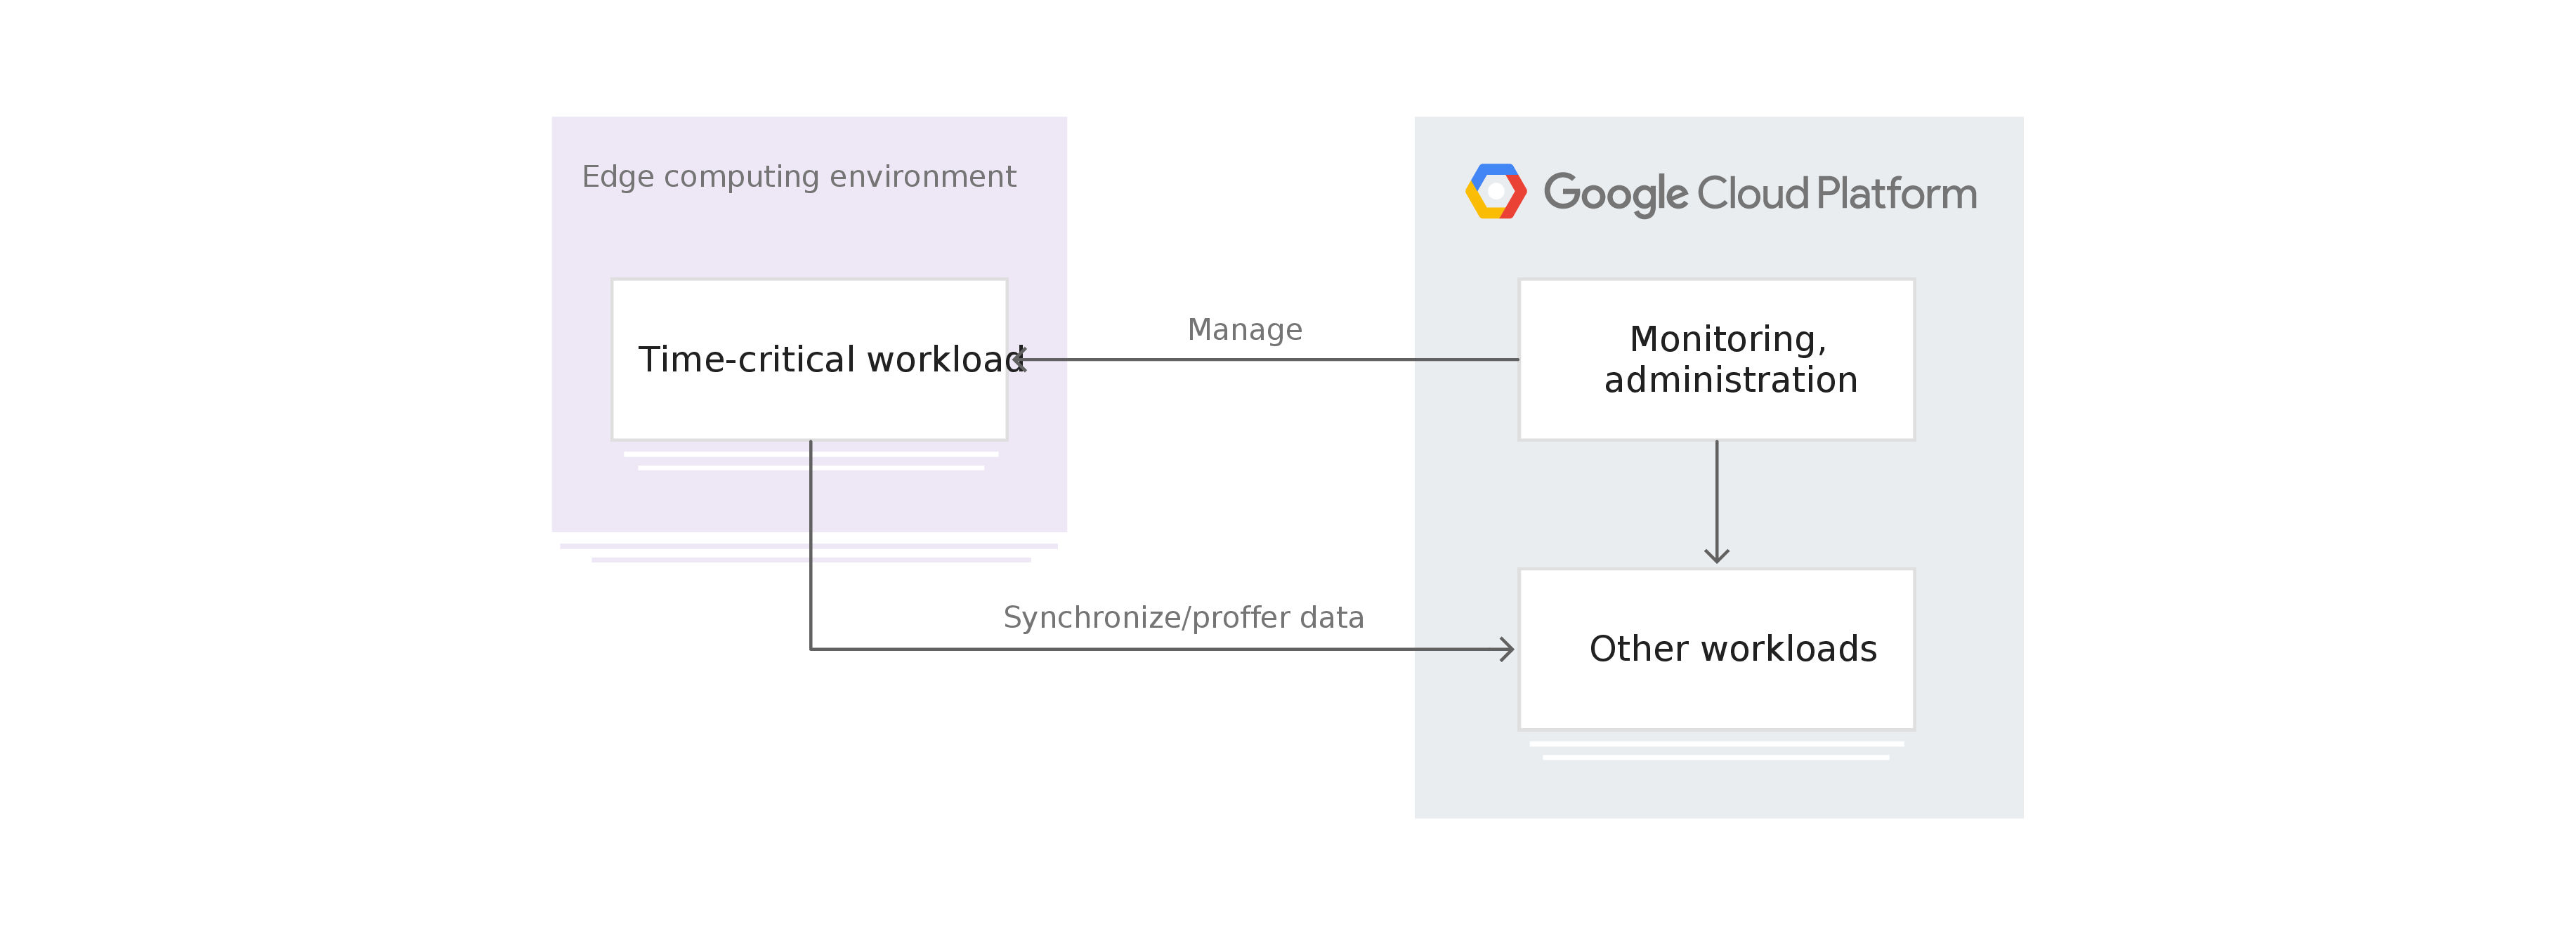
\includegraphics[width=0.8\textwidth]{images/edge.jpg}
    \par
	  \caption{Google edge architektura\label{fig:edge}, zdroj: \source{\cite{edge-picture}}}
    \end{centering}
\end{figure}

Řešení pro správu hybrid cloud prostředí nabízí uživatelům možnost spravovat zdroje různých poskytovatelů z jednoho cetralizovaného místa. Některá řešení jako jsou Red Hat Cloudforms (Manage IQ) a Mist.io se zaměřují primárně na správu infrastruktury u jednotlivých poskytovatelů. Jejich úkolem je připravit infrastrukturu, kam patří fyzické a virtuální servery, uložiště a síťové prvky, pro běh aplikací napříč zdroji \linebreak od více poskytovatelů. Na druhé straně řešení jako Spinnaker, Kubernetes Federation a Cloud foundry se primárně zaměřují na správu aplikací, které běží distribuovaně u více poskytovatelů cloudu. V následující sekci jsou jednotlivá řešení představena detailněji. 


\section{Red Hat Cloudforms/Manage IQ}
Cloudforms je platforma pro jednotnou správu fyzických a virtuálních serverů a také kontejnerů napříč různými cloudovými prostředími. Pomocí CloudForms je možné ovládat zdroje v technologiích pro privátní cloudy OpenStack a také virtuální servery spravované technologií od společnosti VMware, Red Hat virtualization a Microsoft Hyper-V. CloudForms umožňuje spravovat zdroje ve veřejných cloudech AWS (Amazon web services), Microsoft Azure a také GCP (Google cloud platform). CloudForms umožňuje spravovat také kontejnery na platformě OpenShift. CloudForms technologie vychází z Manage IQ technologie. Manage IQ je jednotná open-source platforma pro správu cloudových prostředí. Cloudform je vyvíjeno, spravováno a podporováno přímo společností Red Hat, jedná se o komerční řešení. Manage IQ je stejná platforma s otevřeným kódem, která je spravována a rozvíjena komunitou napříč různými společnostmi \cite{manageiq}. Dále v textu je popisována Manage IQ verze.\par
    Manage IQ přistupuje k jednotlivým systémům, označovaným jako poskytovatelé, přes API, které např. veřejné cloudy nebo OpenStack poskytují. Přes tato API si Manage IQ vyčítá informace o jednotlivých zdrojích  jako jsou virtuální servery, kontejnery, load-balancery společně s jejich metadaty jako jsou jméno, typ a mnoho dalšího. Tyto zdroje jsou označovány jako managed elements, neboli spravovaný prvek, a jsou uloženy ve Virtual Managemet Database (VMDB). Manage IQ po počátečním získání informací z jednotlivých poskytovatelů stále sleduje jednotlivá API poskytovatelů a udržuje VMDB stále aktuální. Manage IQ poskytuje přehledné webové rozhraní ve kterém jsou zobrazeny jednotlivé zdroje poskytovatelů s detailními informacemi.\linebreak Například při připojení na VMware je zobrazen seznam běžících virtuálních serverů společně s jejich atributy jako je počet jader, velikost RAM, operační systém, připojené sítě, nainstalované programy a tak dále. \par
    Manage IQ dovoluje provádět akce nad objekty, které má zaregistrované ve VMDB. Například virtuální servery běžící ve VMware prostředí můžeme vytvářet, mazat, vypínat, zapínat a restartovat. Další oblastí správy zdrojů je sledování a provádění změn. Můžeme sledovat jednotlivé atributy zdrojů a také kdy došlo k jejich změně. Manage IQ umožnuje také porovnávat aktuální stav s počátečním stavem. Např. jaké změny byly provedeny na virtuálním serveru oproti jeho základní konfiguraci. Manage IQ může zaznamenat změnu sudo práv, přidání nového uživatele nebo nainstalování \linebreak nového balíčku. Protože Manage IQ má data o všech zdrojích jednotlivých poskytovatelů, můžeme s jeho pomocí počítat náklady na provoz.\par
    Další věcí, kterou Manage IQ nabízí jsou služby. Služby dovolují vytváření složitějších konfigurací jednoduchou cestou. Přes služby můžeme například vytvořit dva virtuální servery s nainstalovaným webovým serverem, jeden server poběží v prostředí OpenStacku a druhý na VMwaru. Dále virtuální server sloužící jako databáze a poté ještě load-balancer, který bude rozkládat zátěž mezi webové servery. Výběr těchto zdrojů může například sloužit vývojářům aplikace jako prostředí pro vývoj. Vytvořit takovéto prostředí bude možné na jedno kliknutí. Správce vytvoří podle požadavků skript, který tyto zdroje vytvoří a poté zdroje nastaví. Vývojáři mohou z webového rozhraní skript spustit a během chvíle dostanou připravené prostředí pro vývoj. Tento nástroj dovoluje vytvářet složitější konfigurace a jednoduše je nasadit. Vývojáři tak tráví více času programováním aplikace namísto nastavování serverů. Administrátoři mohou povolit přistup k určitým zdrojům pouze uživatelům, kteří splnují stanovená pravidla. Např. pouze uživatelé ve skupině vývojáři mohou spouštět skript, který vytvoří vývojářské prostředí z předchozího příkladu \cite{lwn}.

\section{Cloud foundry}
Cloud Foundry (CF) je open source cloudová PaaS platforma. Na této platformě mohou vývojáři jednoduše vytvořit, nasadit, běžet a škálovat aplikace. CF bylo původně vytvořeno společností VMware. Později došlo ke zveřejnění zdrojových kódů a stalo se komunitním projektem. Jedná se o Paas řešení, které je dobře nastavitelné a rozšiřitelné, uživatelé mohou používat širokou škálu frameworků a programovacích jazyků. CF může být nasazeno na vlastní hardware případně na jinou podporovanou cloud platformu jako je AWS nebo OpenStack. CF poskytuje seznam certifikovaných platforem jako jsou IBM Cloud Foundry, Atos Cloud Foundry nebo Pivotal Cloud Foundry. Tyto certifikované platformy zaručují, že aplikace se budou na těchto platformách chovat stejně. Tento fakt minimalizuje vendor lock-in, tedy upoutání se pouze na jednoho poskytovatele. Další výhodou je možnost využití CF pro provozování aplikací na více cloudech, tedy multi-cloud \cite{cf}.\par
CF se skládá z mnoha komponent a má otevřenou architekturu, které zahrnuje tkz. buildpack mechanismus. Tento mechanismus dovoluje přidávat nové frameworky, aplikační služby a také rozhraní pro cloudové poskytovatele. Prvním komponentou je router, který směruje příchozí požadavky na odpovídající komponenty. Další komponentou je UAA (user account and authentication) server, který vykonává správu identit obsažených v systému a přístup uživatelů k jednotlivým zdrojům. Další důležitou komponentou je Cloud Controller, který zajišťuje nasazení aplikace. Cloud controller řídí Diego Brain komponentu, aby spustila požadovanou aplikaci a společně obstarávají celý životní cyklus aplikace. Diego Brain je komponenta, která spouští jednotlivé aplikace a sleduje zda se aplikace nachází v požadovaném stavu. Diego Brain, implementuje control plane, rozhoduje o tom co a kde bude spuštěno. Pro samotné spuštění je zodpovědná komponenta Diego Cell. Cell jsou virtuální servery, na kterých běží požadované aplikace. Aplikace jsou spouštěny v kontejnerech. CF používá jako běhové kontejnerové prostředí vlastní produkt Garden-runC \cite{garden}, který splňuje OCI standard. Diego Cell poskytuje pro tyto kontejnery statistiky použití, logy a další informace. Další funkcí CF jsou služby. Služby fungují v CF jako katalog, ze kterého si vývojář vybírá. Příkladem může být MySql, Redis, Jenkins, Rabbit MQ a mnoho dalších. Vývojář může využít předem definované zdroje, které společně s jeho aplikací vytvoří vybranou službu, bez nutnosti manuální instalace a konfigurace daného nástroje. CF dovoluje vytvářet a přidávat vlastní služby. Aby mohly být služby uspěšně spuštěny, musí implementovat definované API \cite{pivotal}. \par
    Aby mohlo CF spouštět aplikace na virtuálních serverech, potřebuje ovládat infrastrukturu, která hostuje CF aplikace. K tomuto učelu slouží nástroj BOSH, který \linebreak zaručuje, že prostředí je správně nastavené a připravené hostovat uživatelské aplikace. BOSH se skládá ze tří vrstev. První vrstvou je Stemcell, který představuje univerzální operační systém, který abstrahuje aplikaci od operačního systému serveru, je stejný přes všechny poskytovatele a umožnuje jednotnou správu virtuálních serverů. Druhou vrstvou je vydání (Release), popisuje jaký software by měl být nasazen a jak by měl být nastavený. Druhá vrstva zaručuje opakované spuštění aplikace se stejným výsledkem. Poslední částí BOSH je 
    manifest soubor, který popisuje jaký release by měl být nasazený a do jakého cloudu. BOSH také dovoluje spouštět aplikace v multi cloud prostředí. BOSH používá Cloud provider interface (CPI), aby abstrahoval rozdíly mezi jednotlivými poskytovateli. Díky tomu je možné přidávat nové poskytovatele. BOSH v současnosti může nasadit aplikaci na platformy AWS, Azure, GCC, OpenStack a také VMware \cite{bosh}.

\section{Mist.io}
Mist.io je open-source platforma, která zjednodušuje uživatelům správu cloudu. Mist.io poskytuje jednotné rozhraní pro správu cloudových řešení různých společností. Nástroj Mist.io může spravovat fyzické servery, virtuální servery na technologiích KVM, \linebreak VMware, OpenStack nebo Rackspace. Mist.io ovládá také zdroje největších veřejných cloud poskytovatelů AWS, Google cloud engine a Azure. Mist.io dává uživatelům možnost monitorovat Docker kontejnery. Díky široké podpoře cloudových technologií může být Mist.io využito i pro správu multi-cloud infrastruktury a minimalizovat závislost pouze na jednom poskytovateli. Mist.io je možné využívat ve třech verzích. První verzí je Community edition, která je volně dostupná a uživatelé si ji musejí spravovat sami. Druhou verzí je Enterprise edition, která může být nasazena on premise na privátních serverech společnosti. Tato placená verze zahrnuje profesionální podporu od samotné společnosti Mist.io. Poslední možností je využítí SaaS verze Mist.io produktu. Uživatelé této verze platí pouze za využítí zdrojů a jedná se o nejjednodušší řešení jak s Minst.io začít. SaaS verze poskytuje stejně jako Enterprise edition profesionální podporu. Tato kapitola je vytvořena s využitím oficiální dokumentace k Mist.io nástroji \cite{mistio}.\par
    Mist.io poskytuje webové rozhraní pro správu a monitoring jednotlivých zdrojů \linebreak napříč různými poskytovateli. Součástí aplikace je i API, které umožnuje automatizovat jednotlivé postupy. Prvním krokem je přidání cloudových platforem, které budou \linebreak spravovány. Každý poskytovatel vyžaduje rozdílnou konfiguraci pro správné \linebreak fungování. Například pro správu fyzického serveru je nutné poskytnou ip adresu, ssh klíč, uživatele s root právy a číslo portu pro připojení. Pro připojení AWS poskytovatele je nutné vyplnit API klíč a přístupový klíč. Po přidání jednotlivých poskytovatelů je možné si prohlížet jednotlivé zdroje poskytovatelů a dále s nimi pracovat. Mist.io rozlišuje několik základních zdrojů jako jsou machines, images, networks, keys a scripts. Machines, neboli servery, jsou všechny fyzické a virtuální servery. Ve webovém rozhraní jsou servery jednotlivých poskytovatelů rozlišeny ikonkou. U serverů je možné si prohlížet jejich detaily jako je vytížení procesoru, využití RAM nebo \linebreak zaplněnost disků. Dále je možné spravovat pravidla definovaná pro daný server. \linebreak Pravidla umožnují definovat akci, která se má provést při splnění určitého pravidla. Například pokud služba na serveru neodpovídá, tak dojde k restartu služby. Jednotlivé servery je možné seskupovat do skupin podle tagů, neboli nálepek, a efektivně s nimi pracovat. Mist.io podporuje ssh připojení na vzdálený server přímo z webového prohlížeče. Každý server je možné ovládat pomocí definovaných akcí. Každý poskytovatel nabízí jinou sadu akcí, které je možné vykonávat. Mezi ty základní patří vypnutí, restart a smazání serveru. Jednotlivé servery pak mohou být vytvořeny přímo ve webovém rozhraní nebo přes API. Při vytváření serveru je možné specifikovat jméno serveru nebo poskytovatele, ve kterém bude server spuštěn. Druhým zdrojem jsou images, které slouží pro vytváření serverů nebo kontejnerů. Mist.io zobrazuje images, které objevil v jednotlivých public nebo private poskytovatelích a také z připojeného Docker engine. Součástí kontejner images jsou i základní docker images, které poskytuje přímo Mist.io. Pro další zdroj networks, umožnuje Mist.io zobrazit sítě jednotlivých poskytovatelů společně s informacemi o nich a případně v nich vytvářet subnety.  Aby mohli uživatelé přistupovat přes webové rozhraní na konzoli serverů, Mist.io nabízí možnost spravovat ssh klíče, ty poté přiřazovat jednotlivým zdrojům a získat tak přístup na jejich konzoli. Pokud uživatel klíč nemá, může si ho přes webové rozhraní vytvořit. Posledním zdrojem, který Mist.io nabízí je script. Zdroj script slouží k automatizaci opakujících se ukonů nebo konfiguraci serverů. Jednotlivé script zdroje mohou být vytvořeny v bashových skriptech nebo jako Ansible playbooks. 

\section{Kubernetes federation}
Některé nástroje na správu multi cloud prostředí implementují vlastní řešení jak spravovat Kubernetes clustery napříč různými lokacemi. Kubernetes komunita se také \linebreak rozhodla vyvinout řešení pro správu více clusterů, která je zajímavá pro spoustu \linebreak společností a přidává další možnosti využití. V porovnání s jedním clusterem je nasazení aplikace do více clusterů komplikovanější. Jedním z problémů je, jak bude workload jednotlivých aplikací rozdělován do různých clusterů. Existuje několik možností, replikovat zdroje aplikace mezi všechny clustery, replikovat pouze mezi vybrané clustery nebo zdroje rozdělit mezi jednotlivé clustery. Dále je nutné vyřešit jak bude řízen přistup k jednotlivým clusterům nebo jak postupovat, jestliže vytvářené zdroje nebo jejich část již v nějakém clusteru existují. První verze řešení označovaná jako v1 využila koncept Kubernetes API, aby odstranila jakoukoliv přidanou složitost pro existující uživatele k8s. Tento přístup ovšem nebyl providitelný, protože zahrnoval spoustu problémů jako jsou složitost při znovuvytváření k8s api na úrovní clusteru, omezená flexibilita ve federovaných typech. Jedním z problémů byla také neustálená cesta ke stabilní veřejné dostupnosti (GA verze) a zmatek ohledně k8s API samotného. Například k8s deploymenty jsou veřejně dostupné v kubernetes projektu, ale ve v1 verzi kubernetes federace nebyly dostupné ani v beta verzi. \par
    Původní myšlenka s federací specifické API architektury se dále rozvinula a v současnosti pokračuje jako verze v2. Zatím se jedná pouze o Alfa verzi, která není doporučená používat pro produkční použití. Nový návrh architektury je zobrazen na obrázku \ref{fig:k8s-federated}. Federace může být nastavena pomocí dvou typů informace. Prvním typem je Type configuration, který nám říká, jaké zdroje v API má federace propagovat. Druhým typem je Cluster configuraton, která určuje do kterých clusterů má federace propagovat jednotlivé zdroje. Informace Type configuration se skládá ze tří částí. Template, neboli šablona, obsahuje základní konfiguraci zdroje. Například zdroj FederationReplicaSet obsahuje informace o zdroji ReplicaSet, který má být distribuován do určených clusterů. Druhou částí je Placement, neboli umístění, který říká v jakých clusterech má být zdroj spuštěn. Poslední částí jsou Overrides, které určují specifické parametry pro jednotlivé clustery. Tyto tři části obsahují nejnutnější informace potřebné pro propagaci a jsou navržené tak, aby splňovaly dynamické plánování spouštění zdrojů založené na pravidlech. Další důležité součásti federace k8s jsou Status, Policy a Scheduling. Status shromažduje informace o všech zdrojích spuštěných napříč všemi federovanými clustery. Policy, neboli politiky, rozhodují do jakých clusterů mohou být jednotlivé zdroje distribuovány. Scheduling, neboli plánování, zajišťuje rozdělení jednotlivých workloadů přes různé clustery co nejlépe a nejefektivněji.\par 
        Funkce, které by Kubernetes federace měla poskytovat patří propagace různých typů zdrojů do vzdálených clusterů, CLI nástroj kubefed2 pro správu takovéto federace podobně jako nástroj kubectl, který slouží pro správu jednoho clusteru. Federace by také měla poskytovat DNS a Ingerss služby pro více clusterů. Další funkcí by také mělo být pokročilé nastavení rozmístění jednotlivých zdrojů do clusterů podle uživatelovi preference.


\begin{figure}[H]
  \begin{centering}
	  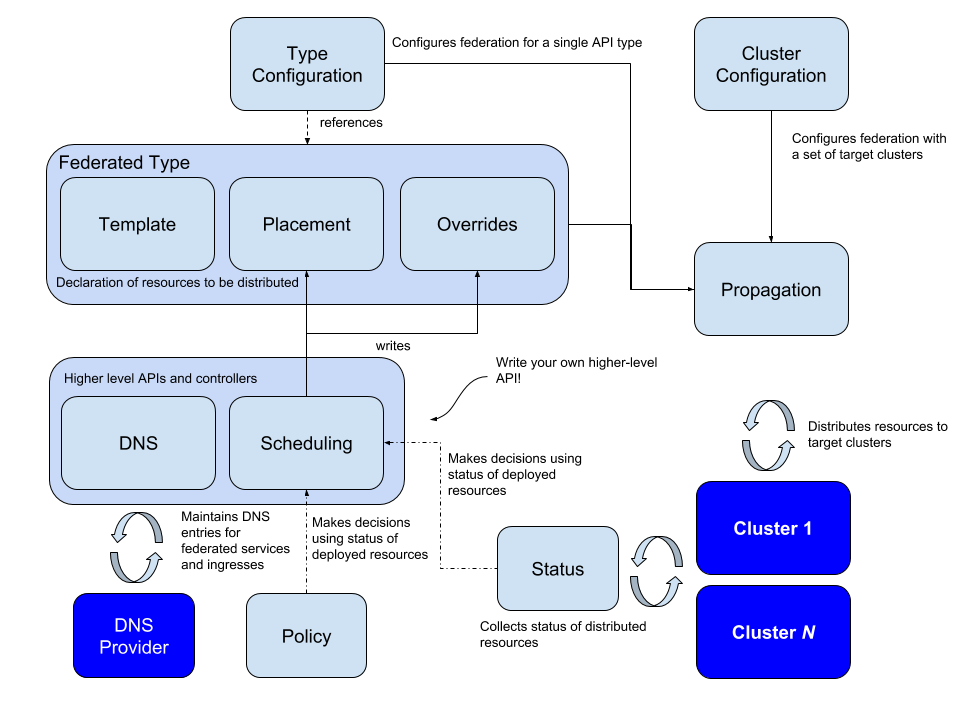
\includegraphics[width=0.8\textwidth]{images/k8s-federated.png}
    \par
	  \caption{Architektura projektu Kubernetes Federation\label{fig:k8s-federated}, zdroj: \source{\cite{federace-picture}}}
    \end{centering}
\end{figure}
	
\section{Spinnaker}
Spinnaker je open source platforma, která umožňuje continuous delivery (CD) aplikací do multi-cloud prostředí. Spinnaker projekt byl vytvořen společností Netflix. Spinnaker je navržen s ohledem na snadnou rozšiřitelnost tak, aby bylo možné přidávat nové cloudové poskytovatele. Spinnaker podporuje nejpoužívanější cloudové poskytovatele jako jsou AWS, Google Cloud, Azure, OpenStack, Oracle Cloud Infrastructure a také technologii Kubernetes \cite{netflix-spinnaker}. Mezi uživatele Spinnakeru patří například Waze, navigační aplikace pro mobilní telefony. Provozovatelé aplikace používají pro běh své aplikace AWS a Google cloud poskytovatele pro vysokou dostupnost své služby a také pro možnosti, které Spinnaker nabízí. Postup, který Waze používá začíná odesláním změn do github repozitáře, Jenkins software vytvoří balíček s požadovanou změnou a spustí další proces, jehož úkolem je nasazení aplikace. V obou cloudech zároveň je vytvořena image s požadovným balíčkem a jsou spuštěny integrační testy. Pokud testy proběhnou bez problémů, aplikace je spuštěna v tesovacím prostředí s reálnými daty. Jestliže aplikace v testovacím prostředí prošla testy je nasazena do produkčního prostředí. V případě chyby může být nová verze stažena z produkce a místo ní nasazena starší stabilní otestovaná verze \cite{waze}.\par
Spinnaker obsahuje dvě základní sady funkcí správu aplikací a nasazení aplikací. S pomocí správy aplikací je možné spravovat a monitorovat zdroje v jednotlivých \linebreak cloudech. Spinnaker vidí aplikace jako jednotlivé microservicy a takto s nimi pracuje. Spinnaker používá k popsání uživatelské aplikace, aplikace kterou chceme pomocí Spinnakeru nasadit do prostředí cloudu, koncepty jako jsou Applications, Clusters a Server Groups. Spinnaker dále používá koncepty Load balancer a Firewall pro popsání jak budou jednotlivé mikroslužby zpřístupněny uživatelům. Koncept Application je ve Spinnakeru reprezentace mikroslužby uživatelské aplikace, její konfigurace a infrastruktury na které bude aplikace provozována. Ač to Spinnaker nevyžaduje, dobrou praxí je vytvoření Spinnaker aplikace pro každou mikroslužbu uživatelské aplikace. Pojem Cluster je označení pro skupinu serverů ve Spinnakeru. Server Groups označení používá Spinnaker pro nasaditelné zdroje jako jsou obrazy virtuálních serverů nebo Docker image a konfiguraci (počet instancí zdroje, metadata, pravidla pro škálování, atd.). Pokud je Server Group nasazena, je kolekcí instací dané mikroslužby (virtuální servery, pody v Kubernetes). Load balancer je použitý pro směrování požadavků mezi instance v jedné Server Group. Load balancer umí také kontrolovat dostupnost \linebreak mikroslužby a v případě poruchy přestat posílat požadavky na poškozený Server Group.\par
Druhá skupina funkcí, kterou Spinnaker nabízí se týká nasazení aplikace a CD (continuous delivery) aplikace. Hlavní částí nasazení aplikace je Pipeline. Pipeline se skládá z posloupnosti akcí, které se označují jako Stages. Pipeline je možné spustit ručně nebo lze nastavit spouštěče. Jako spouštěč mohou být nastaveny různé podněty jako je nový Docker image v Docker registry, dokončení Jenkins úlohy, časový údaj atd. Pipeline také může uživatele upozorňovat o svém spuštění, průběhu, dokončení nebo chybovém hlášení. Stage je atomická část Pipeliny. Jednotlivé Stage se dají různě skládat. Například některá Stage musí být uspěšně dokončena předtím než je spuštěna další. V jiném případě může být spuštěno více Stagí najednou. V rámci jedné Stage může být vytvořen balíček s aplikací, vytvořen Docker image, spuštění testů aplikace nebo  spuštění virtuálního serveru s novou verzí aplikace. Spinnaker využívá cloud native strategie pro správu aplikací. Mezi tyto strategie patří ověřování dostupnosti služeb, nasazení nové verze aplikace společně s blue/green a canary testováním a také možností vrátit předchozí verzi aplikace bez větších komplikací \cite{spinnaker}.

